\documentclass{article}

\usepackage{graphicx}
\usepackage{tikz}
\usepackage{tikzsymbols}
\usetikzlibrary{calc,patterns,shapes.geometric}
\pagestyle{empty}
\usepackage[margin=0pt]{geometry}
\geometry{papersize={14in,12in}}

\def\centerarc[#1](#2)(#3:#4:#5){\draw[#1] ($(#2)+({#5*cos(#3)},{#5*sin(#3)})$) arc (#3:#4:#5);}

\begin{document}
	\begin{figure}
		\centering
		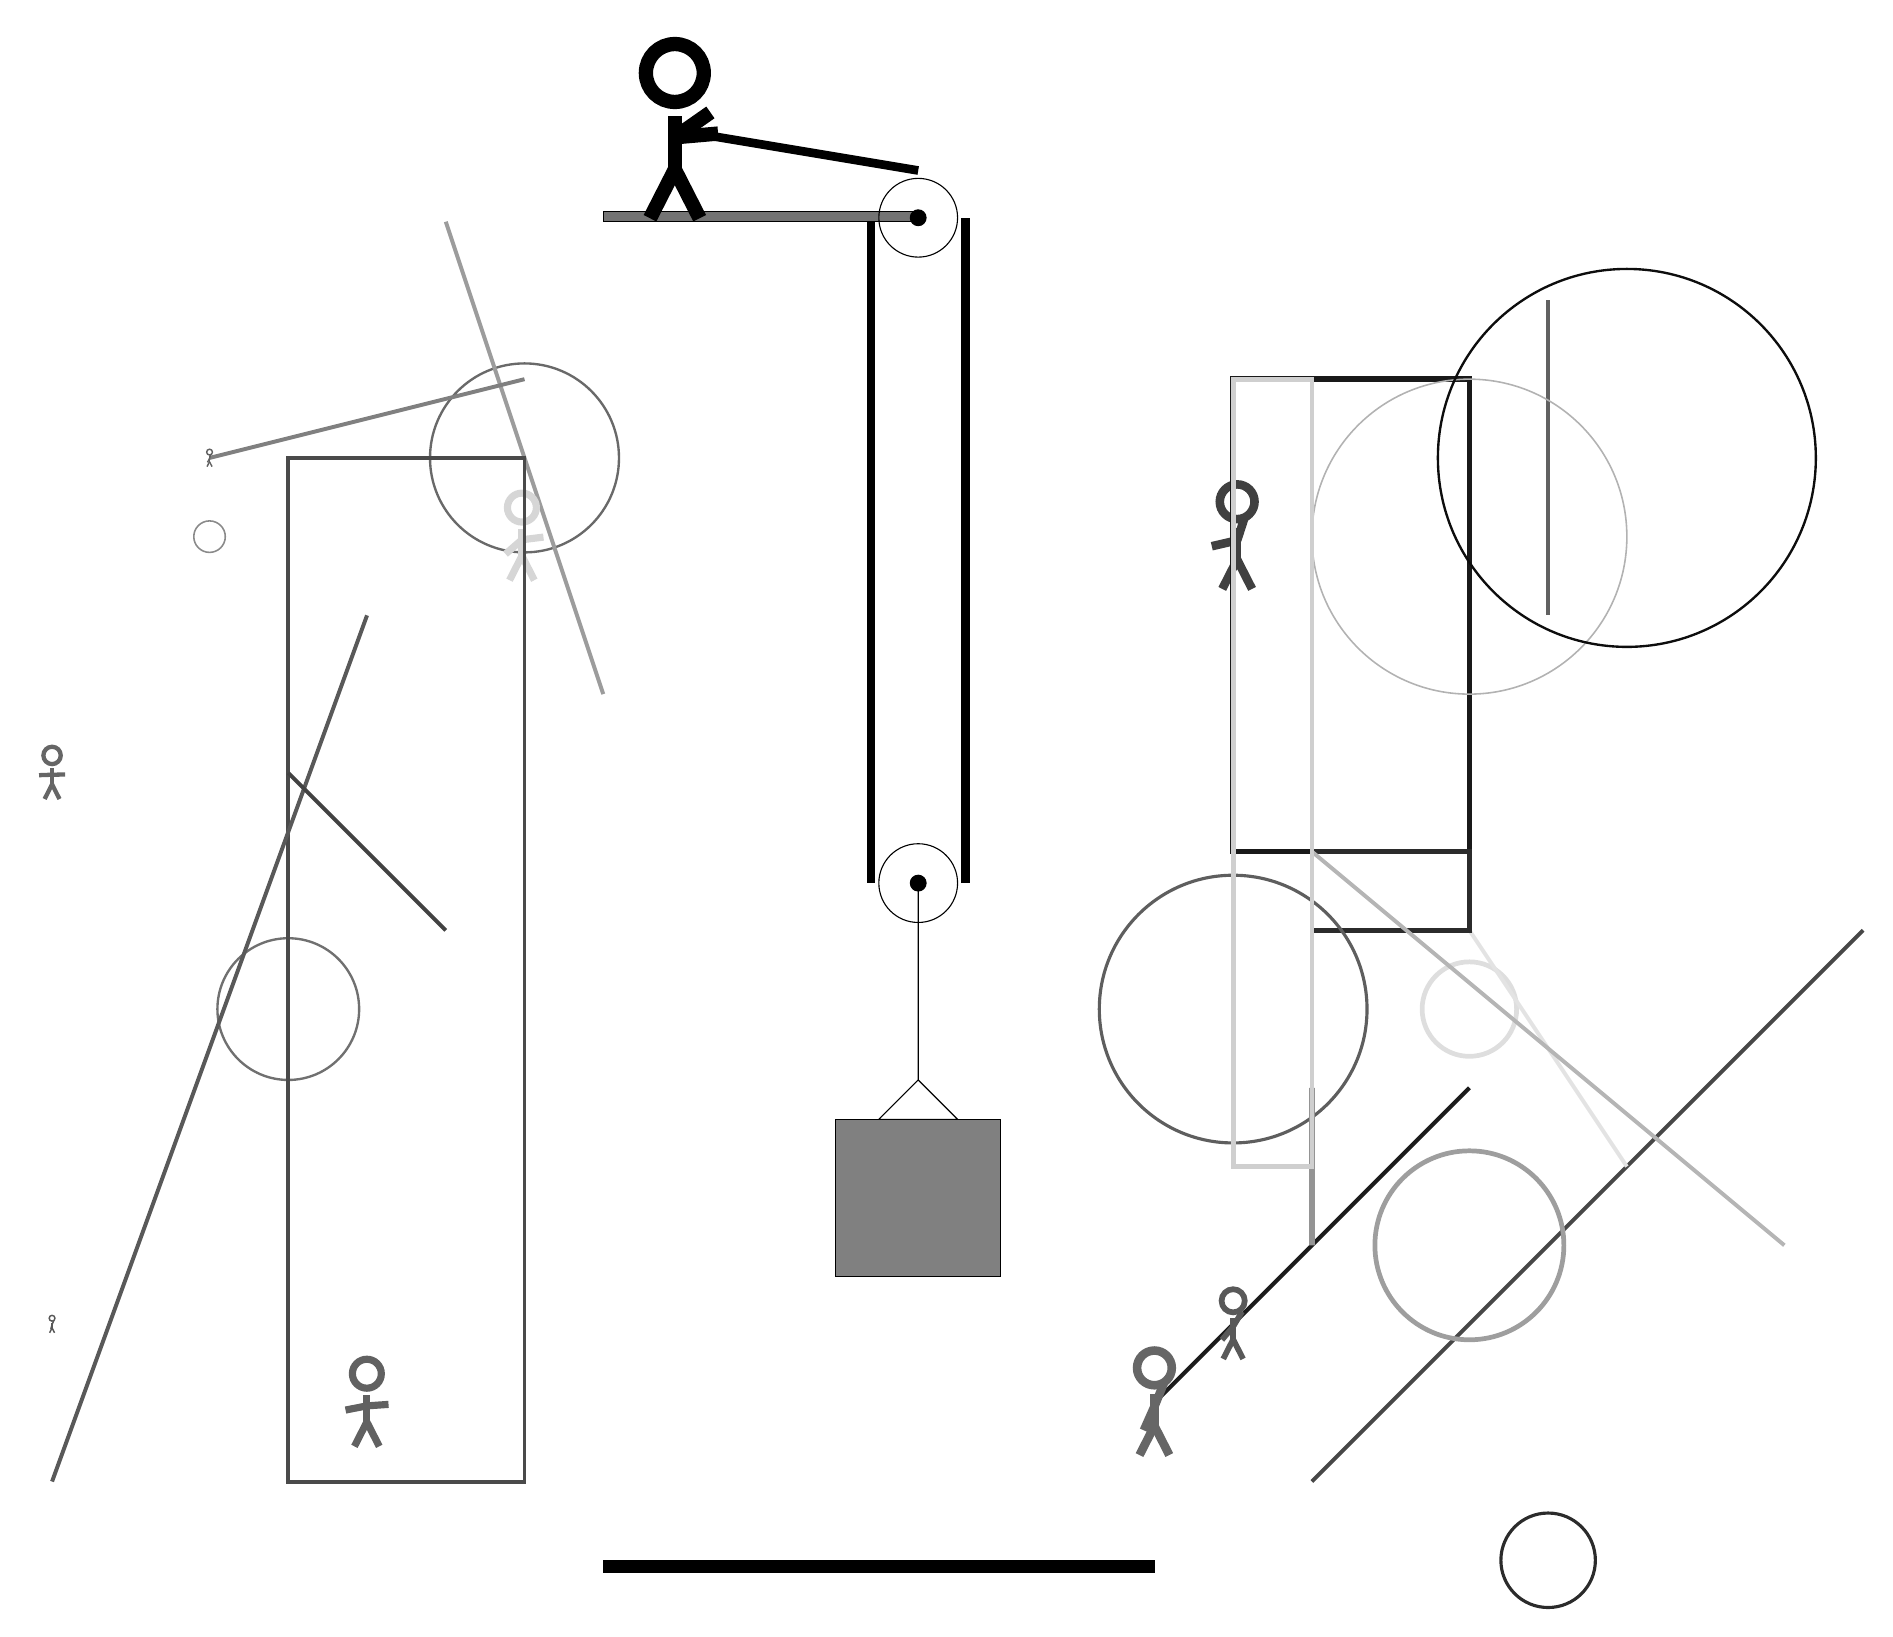
\begin{tikzpicture}
			%%%%% START %%%%%
			
			\draw[fill=black!55] (-2, 14) rectangle (2, 14.125);
			
			\draw (2, 5.6) circle (0.5);
			\draw[fill=black] (2, 5.6) circle (0.1);
			
			\draw (2, 14.05) circle (0.5);
			\draw[fill=black] (2, 14.05) circle (0.1);
			
			\draw (2, 5.6) -- (2, 3.1) -- (1.5, 2.6) -- (2.5, 2.6) -- (2, 3.1);
			\draw[fill=black!50] (0.95, 2.6) rectangle (3.05, 0.6);
			
			\draw[line width=1.1mm] (1.4, 14) -- (1.4, 5.6);
			\centerarc[line width=1.1mm](2, 5.6)(180:360:0.6);
			\draw[line width=1.1mm](2.6, 5.6) -- (2.6, 14.05);
			\centerarc[line width=1.1mm](2, 14.05)(0:90:0.6);
			\draw[line width=1.1mm](2, 14.65) -- (-1, 15.15);
			
			\node at (-1, 15.15) {\Strichmaxerl[10][-175][35]};
			
			\draw [line width=0.3mm, color=black!59](-3, 11) circle (1.2);
			
			\node[line width=0.2mm, color=black!75] at (6, 10) {\Strichmaxerl[6][13][72]};
			\draw[line width=0.5mm, color=black!62](10, 13) -- (10, 9);
			\draw [line width=0.6mm, color=black!13](9, 4) circle (0.6);
			\draw[line width=0.5mm, color=black!72](7, -2) -- (14, 5);
			\draw[line width=0.7mm, color=black!90] (6, 6) rectangle (9, 12);
			
			\draw [line width=0.6mm, color=black!38](9, 1) circle (1.2);
			\draw[line width=0.5mm, color=black!39](-2, 8) -- (-4, 14);
			\draw[line width=0.5mm, color=black!11](9, 5) -- (11, 2);
			\draw[line width=0.6mm, color=black!83] (7, 5) rectangle (9, 6);
			\draw [line width=0.4mm, color=black!63](6, 4) circle (1.7);
			
			\node[line width=0.7mm, color=black!66] at (-9, 0) {\Strichmaxerl[1][73][67]};
			\draw [line width=0.4mm, color=black!83](10, -3) circle (0.6);
			
			\node[line width=0.2mm, color=black!60] at (-9, 7) {\Strichmaxerl[3][2][1]};
			\draw [line width=0.2mm, color=black!30](9, 10) circle (2.0);
			\draw[line width=0.5mm, color=black!89](5, -1) -- (9, 3);
			
			\draw[line width=0.5mm, color=black!29](7, 6) -- (13, 1);
			
			\draw [line width=0.3mm, color=black!56](-6, 4) circle (0.9);
			\draw[line width=0.7mm, color=black!42] (7, 3) rectangle (7, 1);
			\node[line width=0.3mm, color=black!16] at (-3, 10) {\Strichmaxerl[5][41][7]};
			\draw[line width=0.5mm, color=black!50](-3, 12) -- (-7, 11);
			
			\draw[line width=0.5mm, color=black!71] (-3, -2) rectangle (-6, 11);
			
			\draw[line width=0.6mm, color=black!19] (7, 12) rectangle (6, 2);
			\draw [line width=0.2mm, color=black!46](-7, 10) circle (0.2);
			\node[line width=0.5mm, color=black!62] at (-7, 11) {\Strichmaxerl[1][61][74]};
			
			\draw[line width=0.5mm, color=black!65](-5, 9) -- (-9, -2);
			
			\draw [line width=0.3mm, color=black!95](11, 11) circle (2.4);
			\node[line width=0.7mm, color=black!62] at (-5, -1) {\Strichmaxerl[5][11][4]};
			\node[line width=0.3mm, color=black!60] at (5, -1) {\Strichmaxerl[6][66][68]};
			\node[line width=0.3mm, color=black!65] at (6, 0) {\Strichmaxerl[4][50][59]};
			\draw[line width=0.5mm, color=black!74](-6, 7) -- (-4, 5);
			
			
			\draw[fill=black] (-2, -3) rectangle (5, -3.15);
			
			%%%%% END %%%%%
		\end{tikzpicture}
	\end{figure}	
\end{document}